\chapter{E-Government Development Index}
\label{egdi}

\cite{martinez2022egovernment} anuncia 4 tipos de índices de governo eletrônico: EGDI da ONU, GTMI do Banco Mundial, DESI da Comissão Europeia da União Europeia e DGI da OECD.

A não escolha do DESI foi motivada, principalmente, pelo seu escopo. Conforme \cite{desi_2022} explica, o índice é administrado pela Comissão Europeia e foca na análise individual de cada Estado-membro para identificar áreas prioritárias.

Como os foco da análise é o Brasil, o fato do DESI ter sua abrangência limitada a União Europeia afastou a possibilidade de seu uso. Contrariamente, o EGDI, GTMI e DGI têm abrangência global.

Escolheu-se qual índice usar pela quantidade de resultados retornados no Google Acadêmico. A figura mostra a distribuição dos resultados.

\begin{figure}[H]
	\centering
	\caption{Distribuição da quantidade de buscas encontradas dos EGDI, GTMI e DGI}
	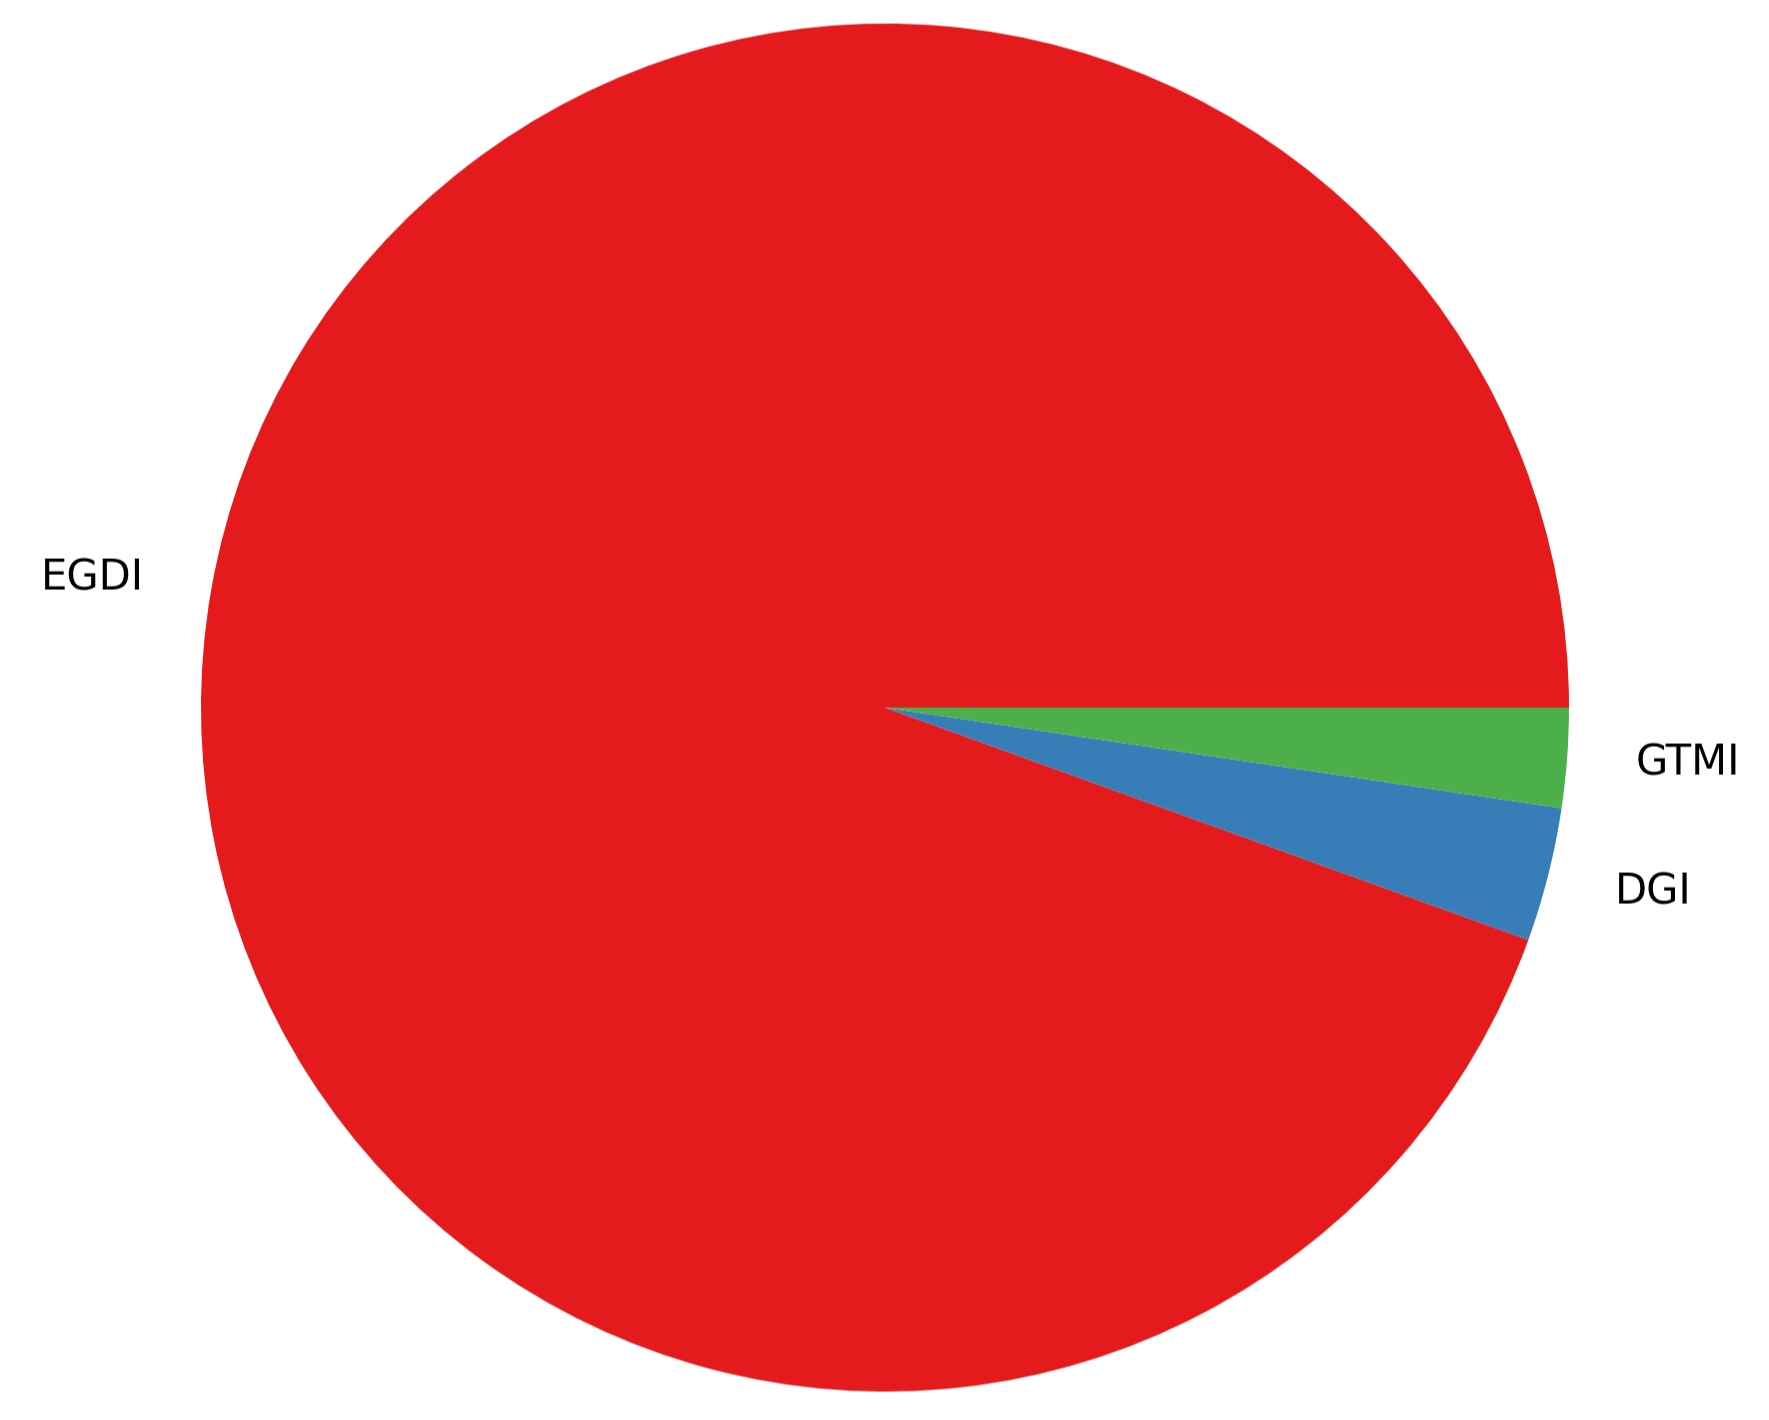
\includegraphics[width=1\linewidth]{figuras/indices/indices_google_academico}
	\label{fig:indices_google_academico}
	\\ \footnotesize{Fonte: elaboração própia.}
\end{figure}

Dentre os índices com abrangência global – EGDI, GTMI e DGI – optou-se pelo primeiro. Embora o GTMI do Banco Mundial e o DGI da OECD também ofereçam visões valiosas sobre a maturidade do governo digital, o EGDI da ONU foi o escolhido devido a maior quantidade de material .

O EGDI apresenta o estado de desenvolvimento de governo eletrônico dos Estados membros da ONU. O índice incorpora as características de acesso, tais como níveis de infraestrutura e educacional para mostrar como um país está usando as tecnologias de informação para promover acesso e inclusão do seu povo \cite{ONU_EGDI}.

\cite{ONU_EGDI} afirma que o EGDI é uma mensuração composta formada por 3 importantes dimensões do governo eletrônico: provisão de serviços online, conectividade de telecomunicação e capacidade humana.

Os componentes do EGDI são:

\begin{figure}[H]
	\centering
	\caption{Os três componentes do EGDI}
	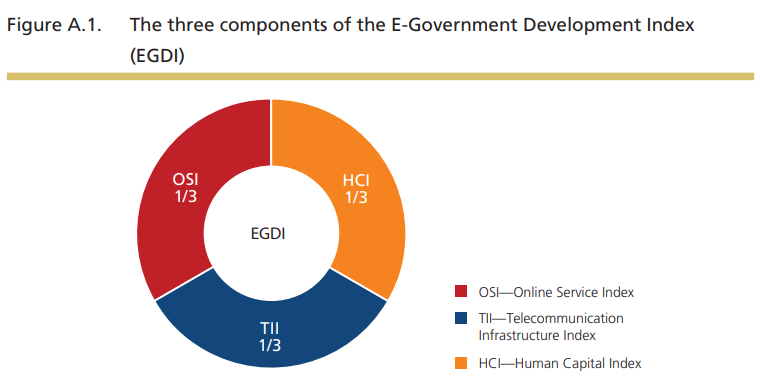
\includegraphics[width=1\linewidth]{figuras/egdi/egdi_componentes.png}
	\label{fig:egdi_componentes}
	\footnotesize{Fonte: \cite{ONU_EGDI_methodology}}
\end{figure}

A figura \ref{fig:boxplot_egov_global} contém um diagrama de caixa que representa o EGDI global.

\begin{figure}[H]
	\centering
	\caption{E-Government Development Index global em 2024}
	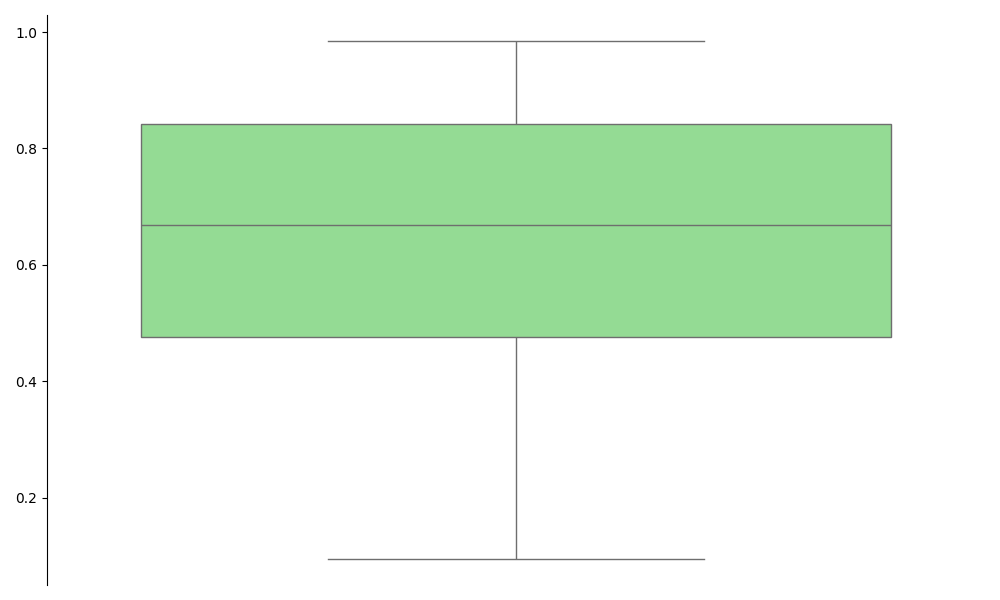
\includegraphics[width=1\linewidth]{figuras/egdi/boxplot_egov_global.png}
	\label{fig:boxplot_egov_global}
	\footnotesize{Fonte: baseado em \cite{ONU_EGDI_mapa}.}
\end{figure}

Os valores mínimo e máximo são, respectivamente, 0.09 e 0.98. O  valor médio é 0.67. Os 1º e 3º quartis são, respectivamente, 0.48 e 0.84.

\section{E-Participation Index}
\label{epart}

\cite{ONU_EGDI} argumenta que o \textbf{E-Participation Index} deriva do EGDI como índice suplementar ao relatório \textbf{E-Government Survey}. Os componentes do índice são: \textbf{E-information}, \textbf{E-consultation} e \textbf{E-decision-making}. 

\textbf{E-information} fala sobre a facilitação da participação dos cidadãos via informações públicas e acesso a informação sem necessidade de pedido ou sob demanda. \textbf{E-consultation} diz respeito ao engajamento dos cidadãos em contribuições e deliberações sobre políticas publicas e serviços públicos. \textbf{E-decision-making} engloba o empoderamento dos cidadãos via a opção de coparticipação na elaboração de políticas e coprodução de componentes de serviços e entrega de modalidades.

\cite{ONU_EGDI} esclarece que o \textbf{E-Participation Index} de um país reflete os mecanismos do índice que são empregados pelo governo quando se faz comparações com todos outros países. 

O propósito dessa medição não é prescrever qualquer prática especificam, no entanto oferece perspectivas de como países diferentes estão usando ferramentas online para promover interação entre o governo e seu povo, bem como, entre as pessoas para benefícios de todos.

A figura \ref{fig:boxplot_epart_global} contém um diagrama de caixa que representa o \textbf{E-Participation Index} global.

\begin{figure}[H]
	\centering
	\caption{E-Participation Index global em 2024}
	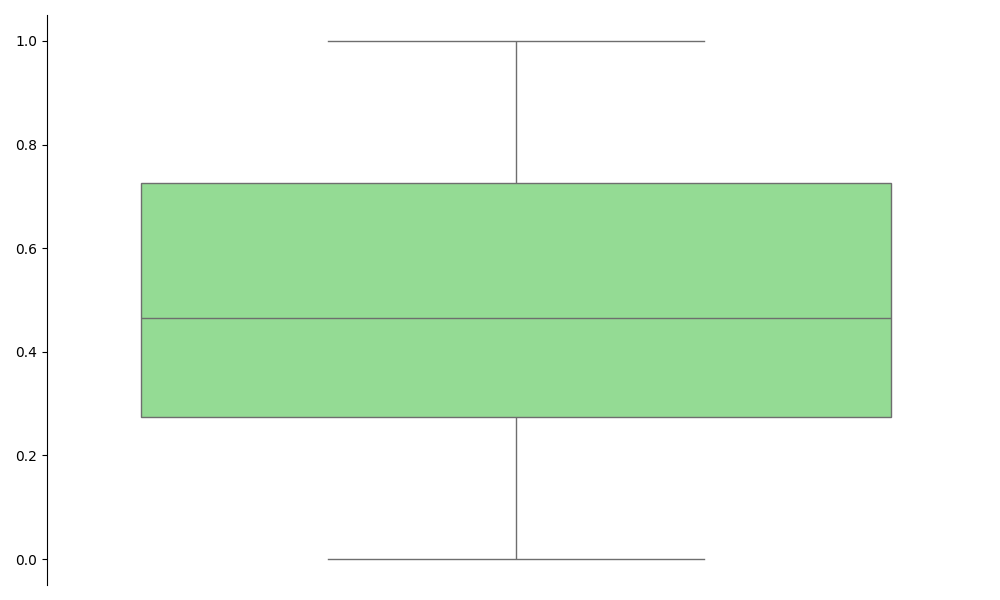
\includegraphics[width=1\linewidth]{figuras/egdi/boxplot_epart_global.png}
	\label{fig:boxplot_epart_global}
	\footnotesize{Fonte: baseado em \cite{ONU_EGDI_mapa}.}
\end{figure}

Os valores mínimo e máximo são, respectivamente, 0.0 e 1.0. O  valor médio é 0.47. Os 1º e 3º quartis são, respectivamente, 0.27 e 0.73.

\section{Online Service Index}
\label{osi}

A figura \ref{fig:boxplot_osi_global} contém um diagrama de caixa que representa o \textbf{E-Participation Index} global.

\begin{figure}[H]
	\centering
	\caption{Online Service Index global em 2024}
	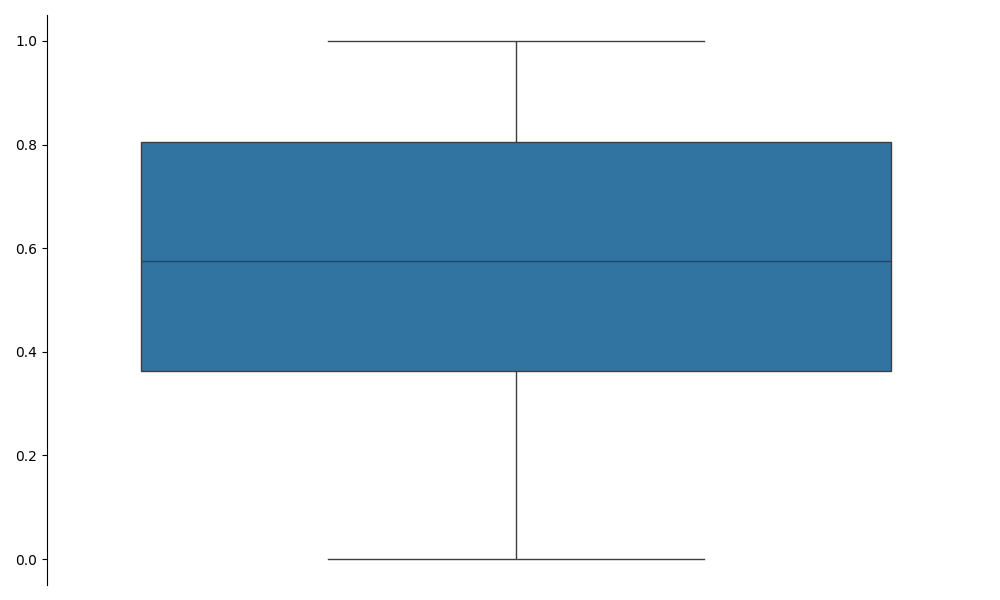
\includegraphics[width=1\linewidth]{figuras/egdi/boxplot_osi_global.png}
	\label{fig:boxplot_osi_global}
	\footnotesize{Fonte: baseado em \cite{ONU_EGDI_mapa}.}
\end{figure}

Os valores mínimo e máximo são, respectivamente, 0.0 e 1.0. O  valor médio é 0.58. Os 1º e 3º quartis são, respectivamente, 0.36 e 0.81.

\section{Human Capital Index em 2024}
\label{hci}

\cite{ONU_EGDI_methodology} afirma que \textbf{Human Capital Index} tem 4 indicadores: taxa bruta de matrícula, letramento adulto, anos de escolarização esperados e média de anos de escolaridade. 

A taxa bruta de matrícula é medida como a combinação entre a taxa de matrícula nas educações primárias, secundários e terciárias. Letramento adulto é medido como o percentual de pessoas com pelos menos 15 anos de idade que entendem e sabem ler e escrever um frase curta simples na sua vida padrão.

Os anos de escolarização esperados é o número total de anos de escolarização que crianças de certa idade podem esperar ter no futuro, presumindo que a probabilidade de a criança de qualquer idade estiver na escola correspondendo à idade da taxa de matrícula atual.

A média de anos de escolaridade fornece o número médio de anos de educação concluídos pela população adulta de um país (25 anos ou mais), excluindo os anos gastos repetindo séries. 

A figura \ref{fig:boxplot_hci_global} contém um diagrama de caixa que representa o \textbf{E-Participation Index} global.

\begin{figure}[H]
	\centering
	\caption{Human Capital Index global em 2024}
	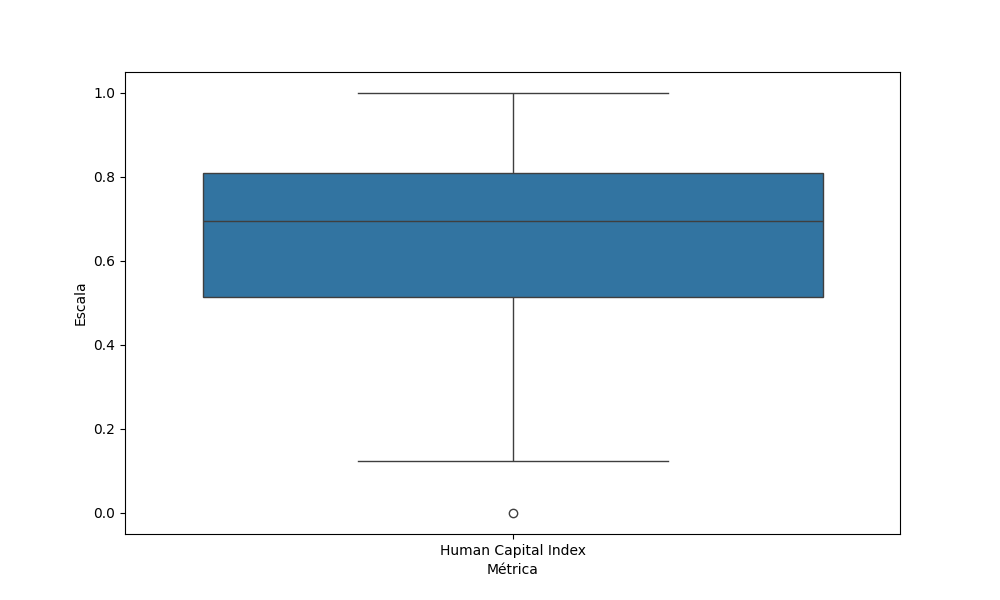
\includegraphics[width=1\linewidth]{figuras/egdi/boxplot_hci_global.png}
	\label{fig:boxplot_hci_global}
	\footnotesize{Fonte: baseado em \cite{ONU_EGDI_mapa}.}
\end{figure}

Os valores mínimo e máximo são, respectivamente, 0.0 e 1.0. O  valor médio é 0.7. Os 1º e 3º quartis são, respectivamente, 0.51 e 0.81.

\section{Telecommunication Infrastructure Index em 2024}
\label{tii}

\cite{ONU_EGDI_methodology} afirma que o \textbf{Telecommunication Infrastructure Index} tem 5 componentes: usuário de internet, assinatura de banda larga fixa, assinatura de banda larga sem fio, assinatura de telefone fixo e assinatura de dados móveis.

A figura \ref{fig:boxplot_tci_global} contém um diagrama de caixa que representa o \textbf{E-Participation Index} global.

\begin{figure}[H]
	\centering
	\caption{Telecommunication Infrastructure Index global em 2024}
	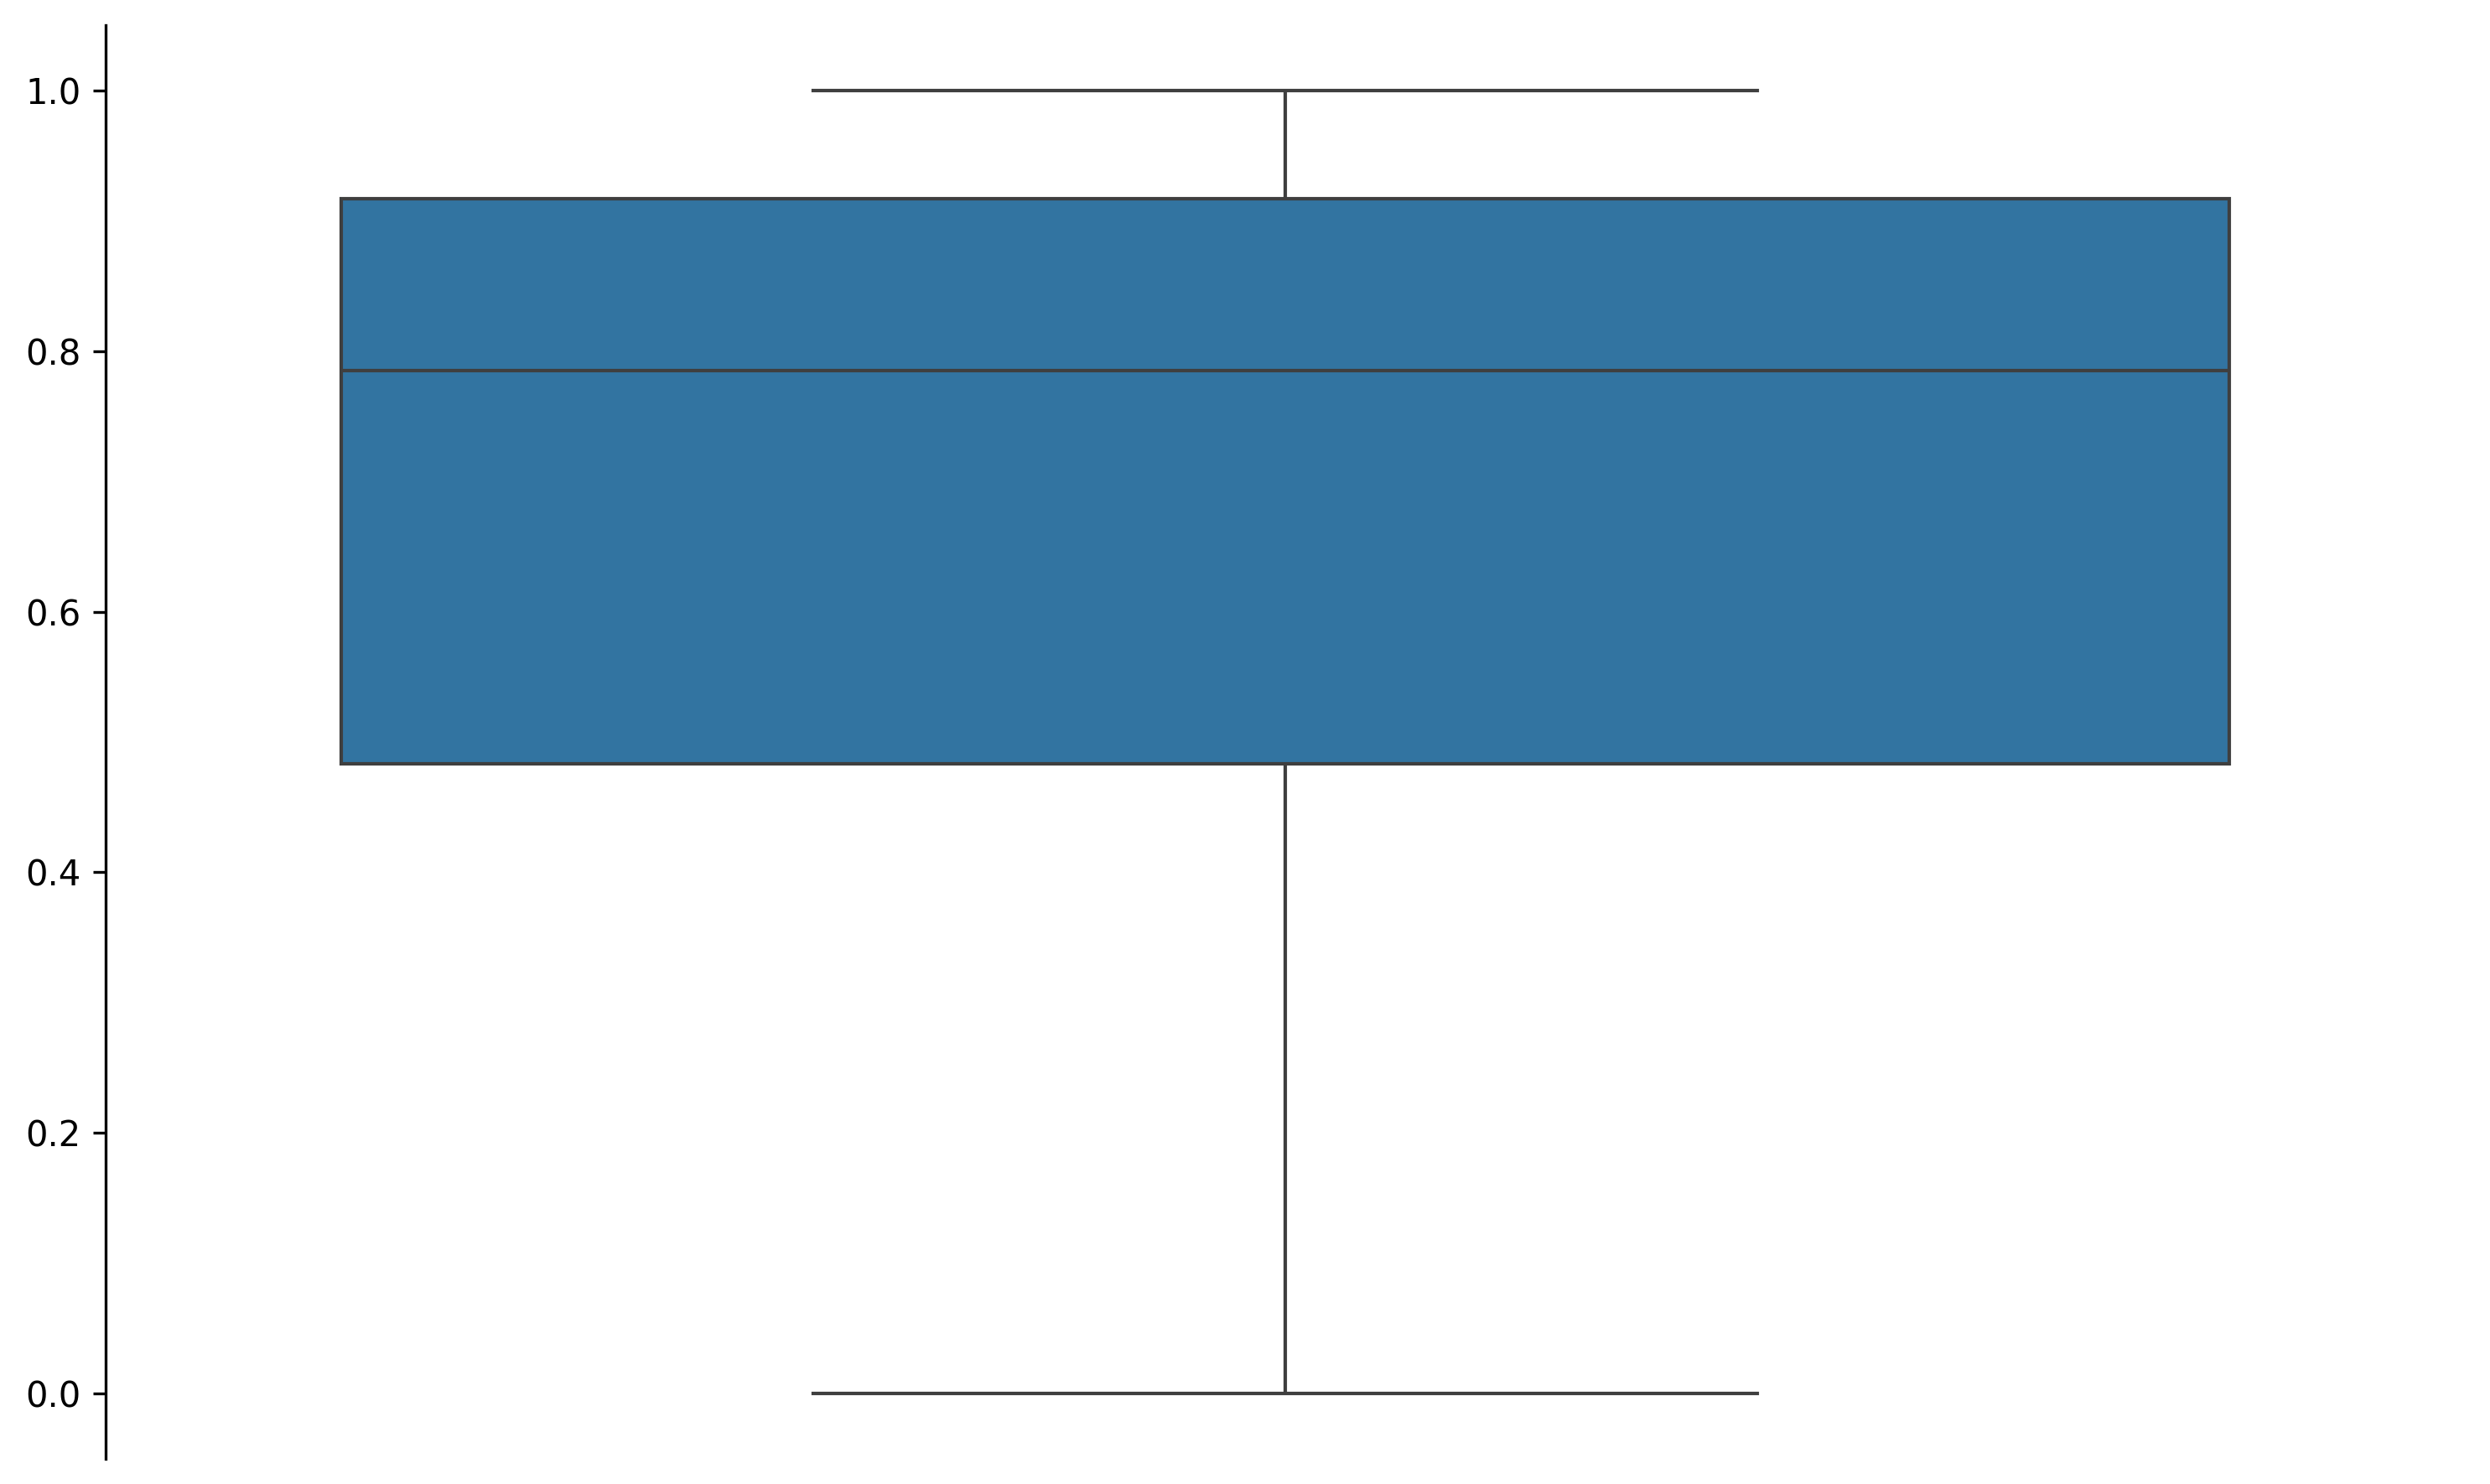
\includegraphics[width=1\linewidth]{figuras/egdi/boxplot_tci_global.png}
	\label{fig:boxplot_tci_global}
	\footnotesize{Fonte: baseado em \cite{ONU_EGDI_mapa}.}
\end{figure}

Os valores mínimo e máximo são, respectivamente, 0.0 e 1.0. O  valor médio é 0.79. Os 1º e 3º quartis são, respectivamente, 0.48 e 0.92.

\section{Coeficiente de correlação: EGDI, seus componentes e E-Participation comparados com o PIB \textit{per capita} PPC e os gastos públicos (\% do PIB)}

\textbf{COMENTARA QUI}

\begin{figure}[H]
	\centering
	\caption{Índice de democracia eleitoral}
	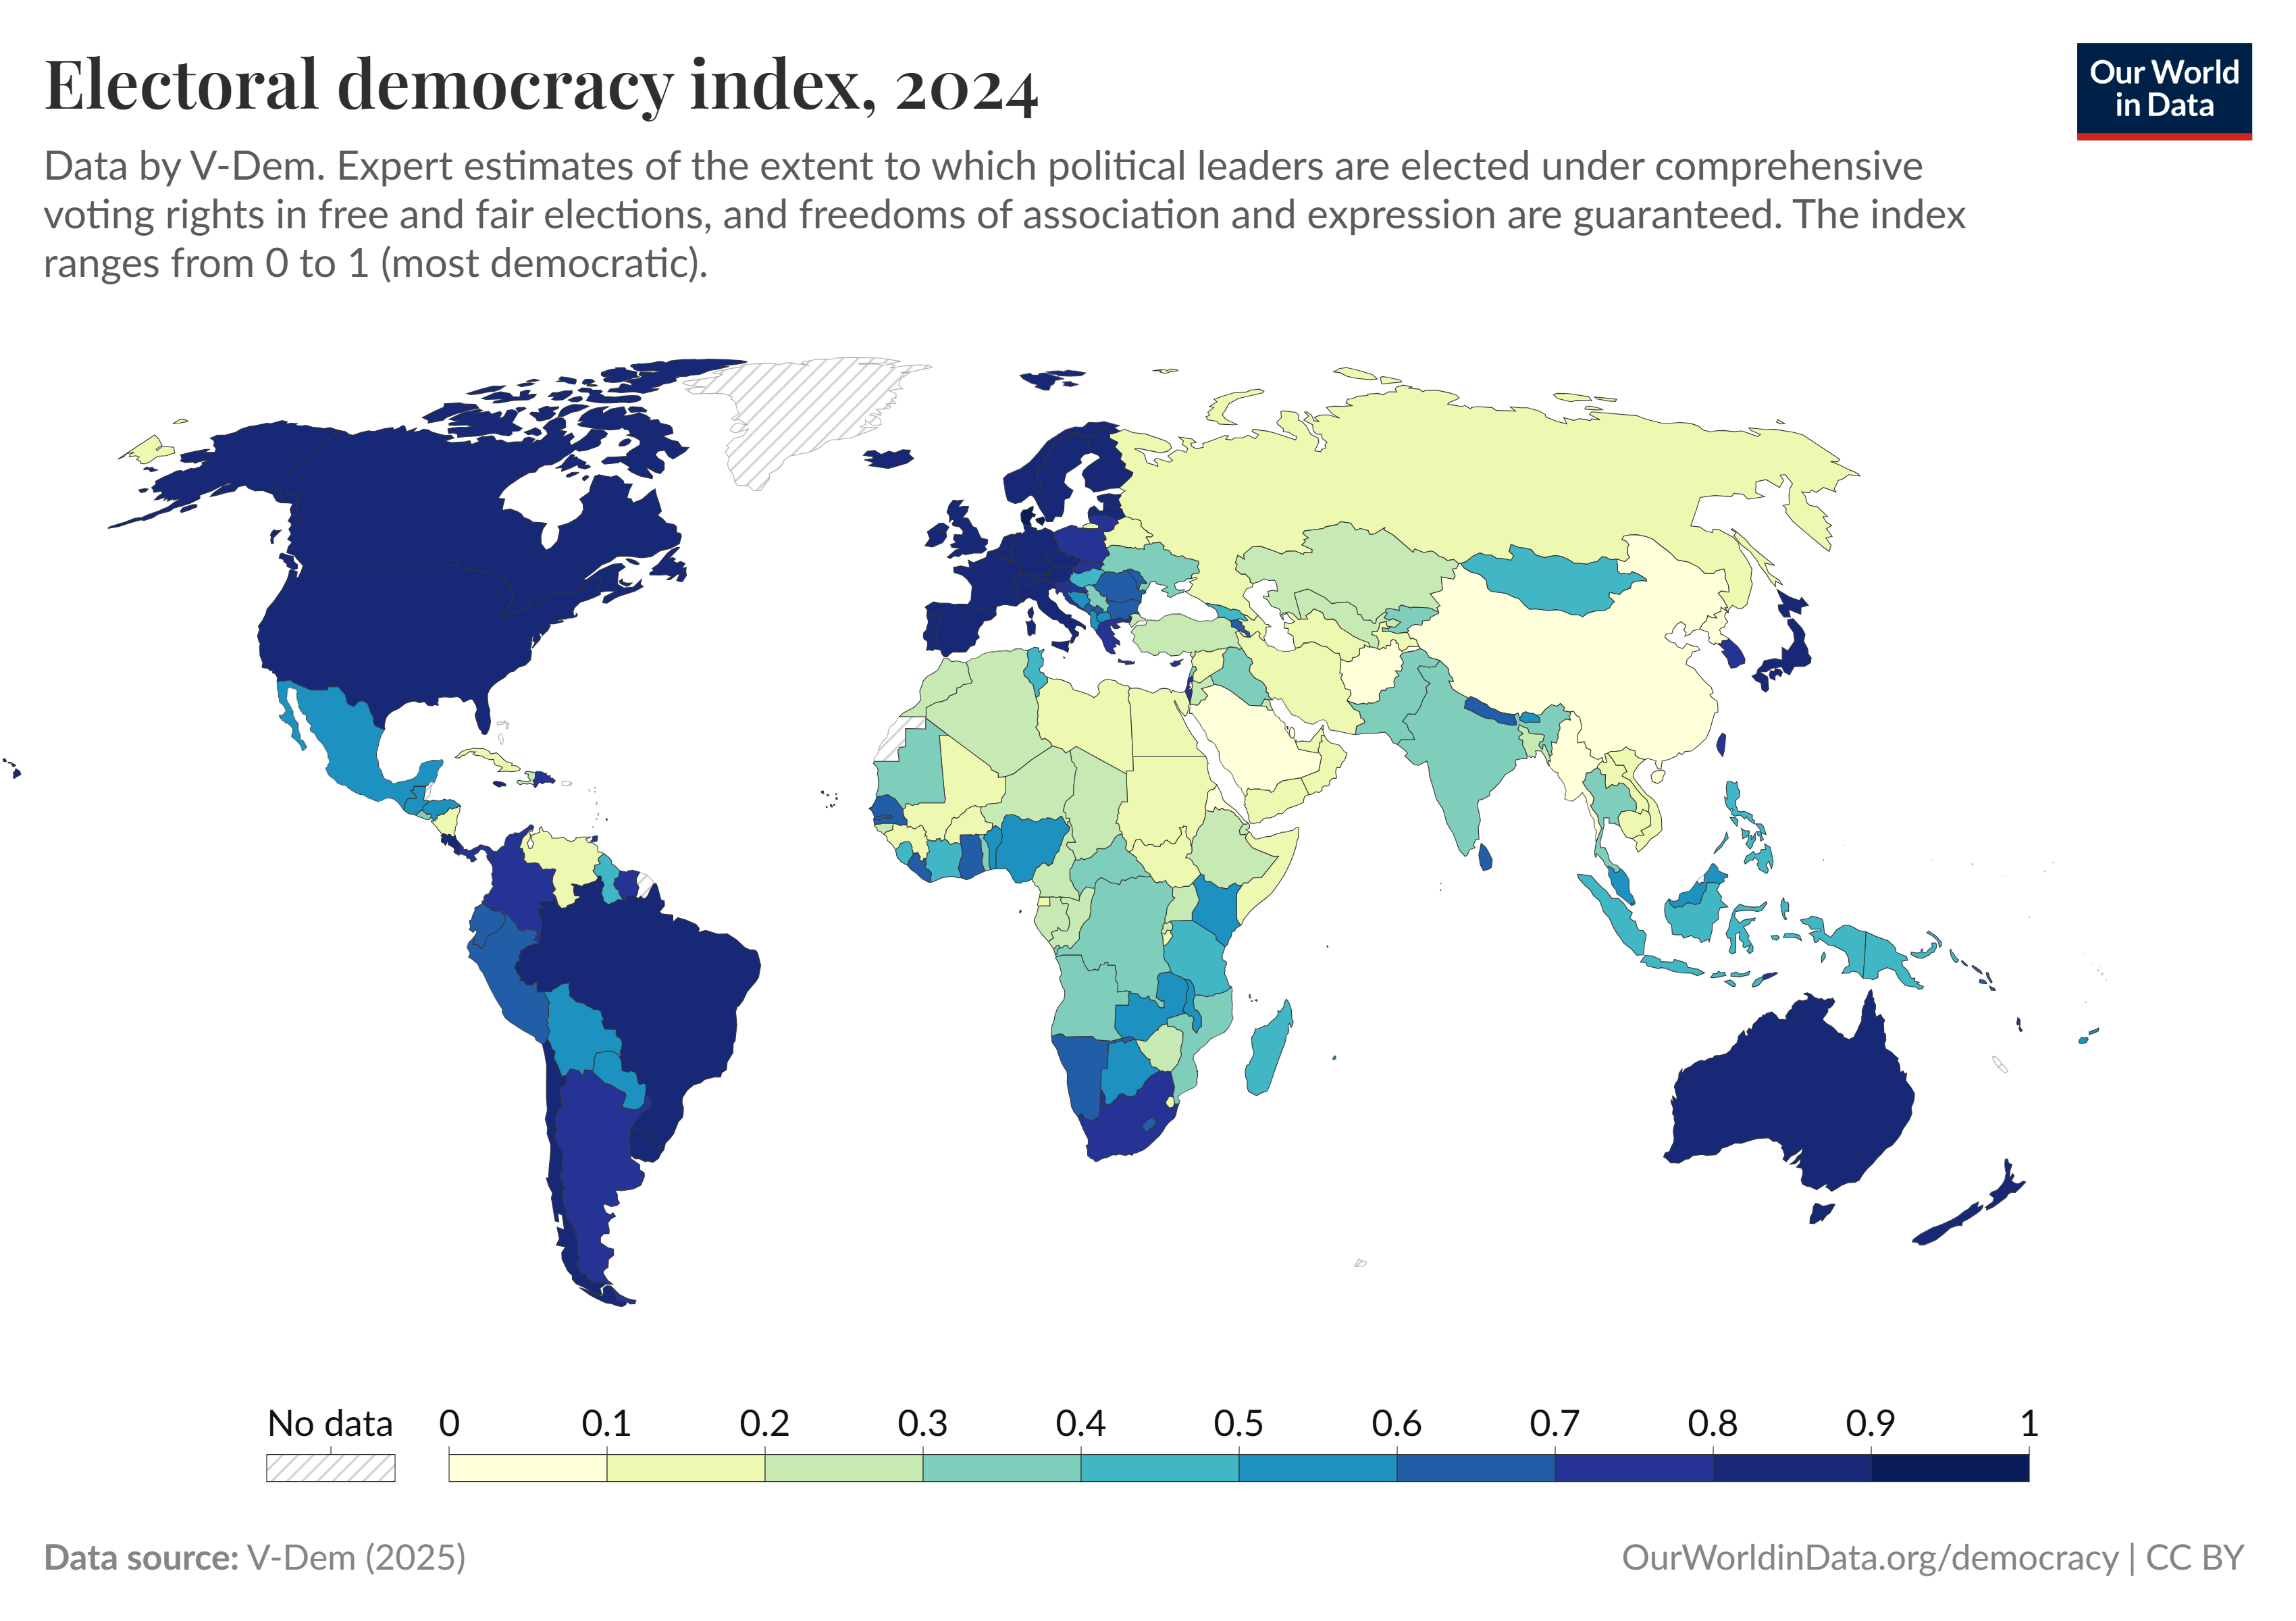
\includegraphics[width=1\linewidth]{figuras/democracia/electoral-democracy-index}
	\label{fig:electoral-democracy-index}
	\footnotesize{Fonte: \cite{electoral-democracy-index}.}
\end{figure}

\begin{figure}[H]
	\centering
	\caption{EGDI no mundo}
	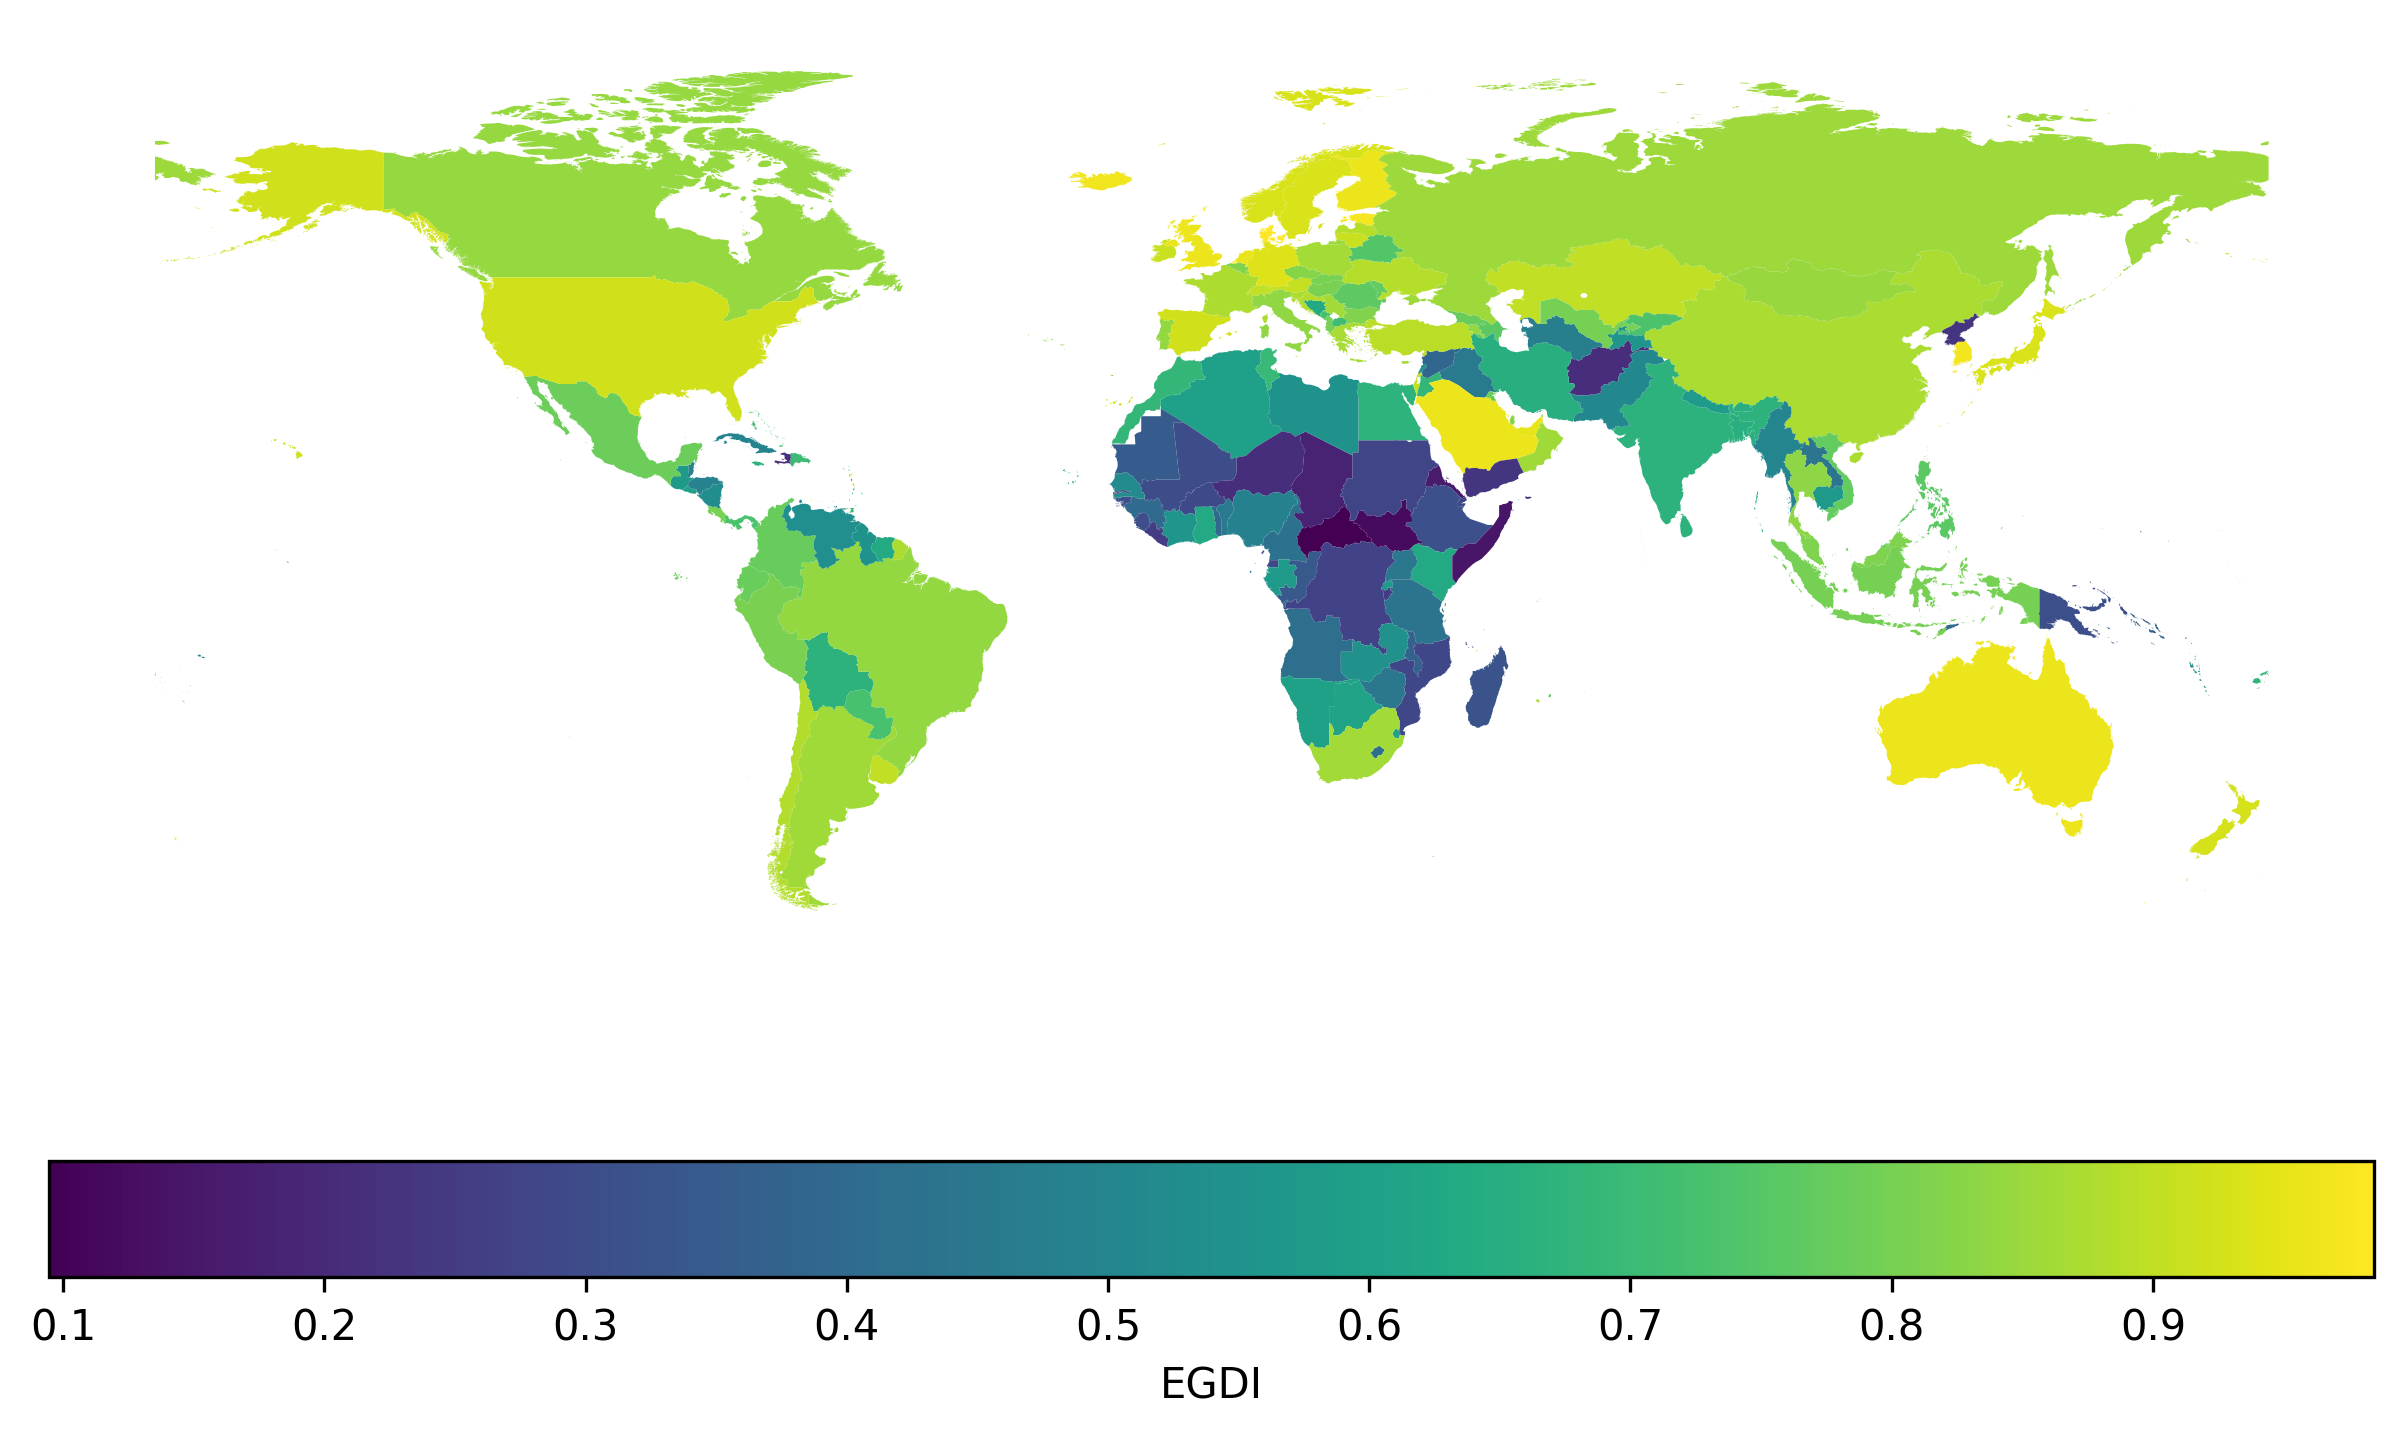
\includegraphics[width=1\linewidth]{figuras/egdi/mapa_coropleto_paises_egdi}
	\label{fig:mapa_coropleto_paises_egdi}
	\footnotesize{Fonte: \cite{ONU_EGDI_mapa}.}
\end{figure}

\begin{figure}[H]
	\centering
	\caption{Gastos públicos no mundo}
	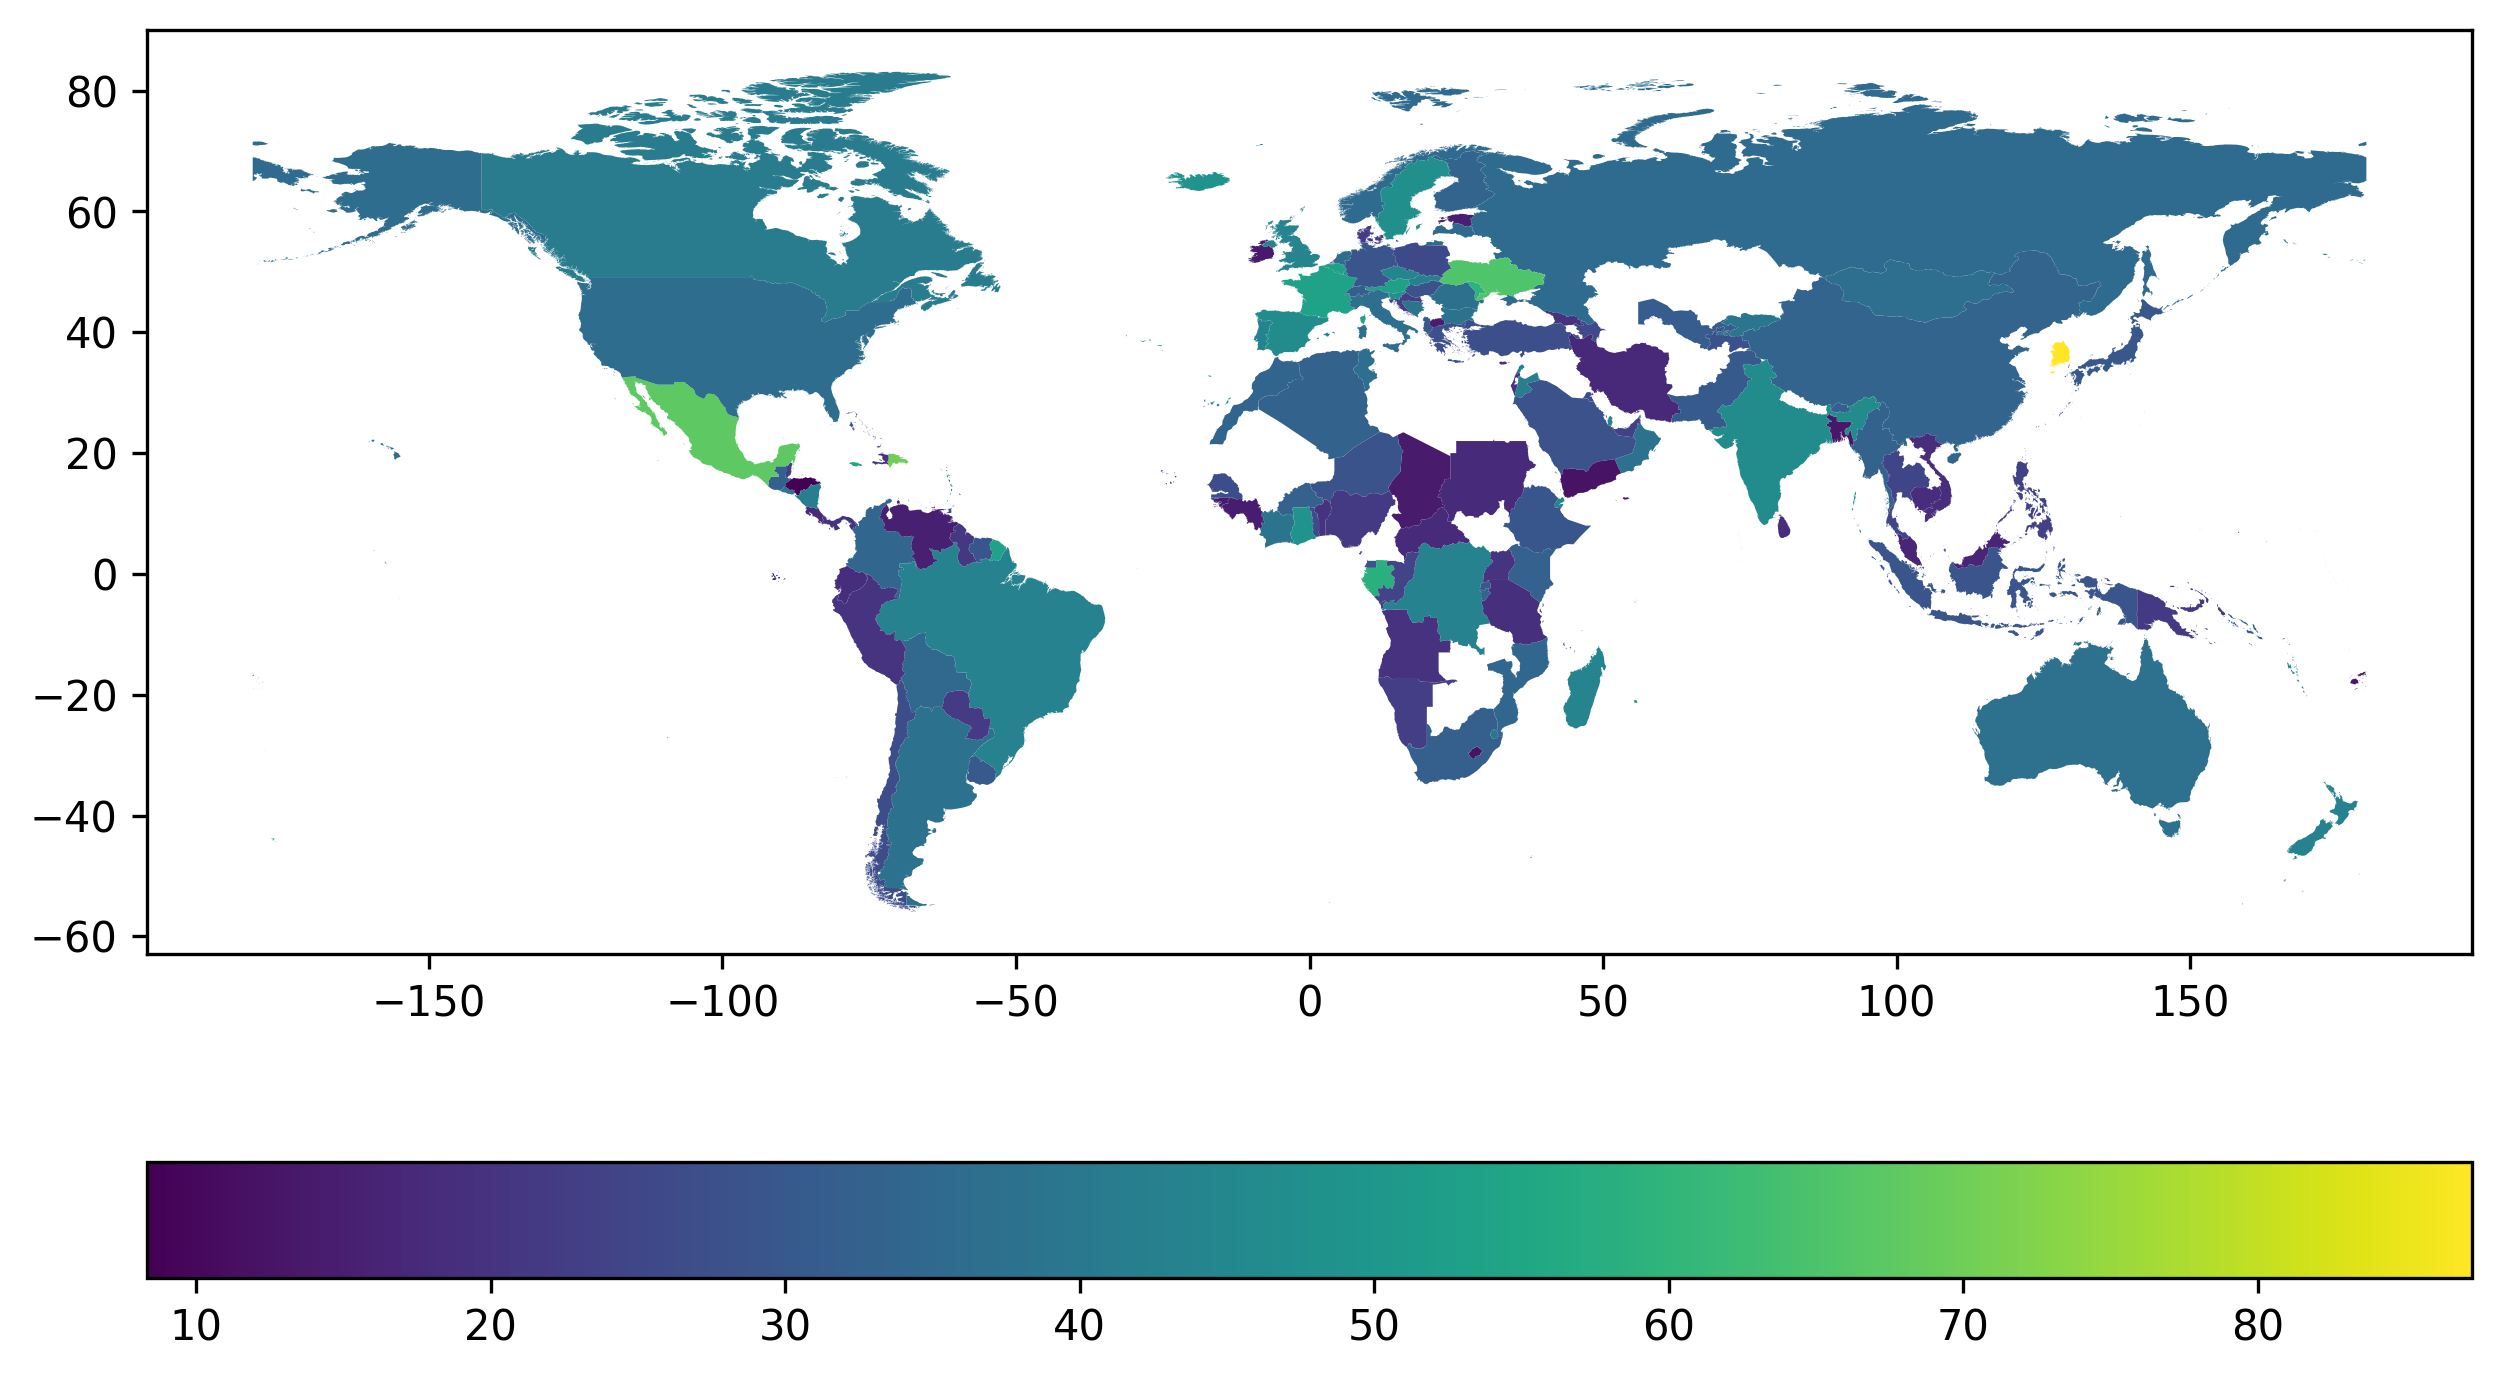
\includegraphics[width=1\linewidth]{figuras/government_spending/mapa_coropleto_paises_gastospublicos}
	\label{fig:mapa_coropleto_paises_gastospublicos}
	\footnotesize{Fonte: \cite{FMI_gov_expenditure}.}
\end{figure}

\begin{figure}[H]
	\centering
	\caption{PIB \textit{per capita} PPC no mundo}
	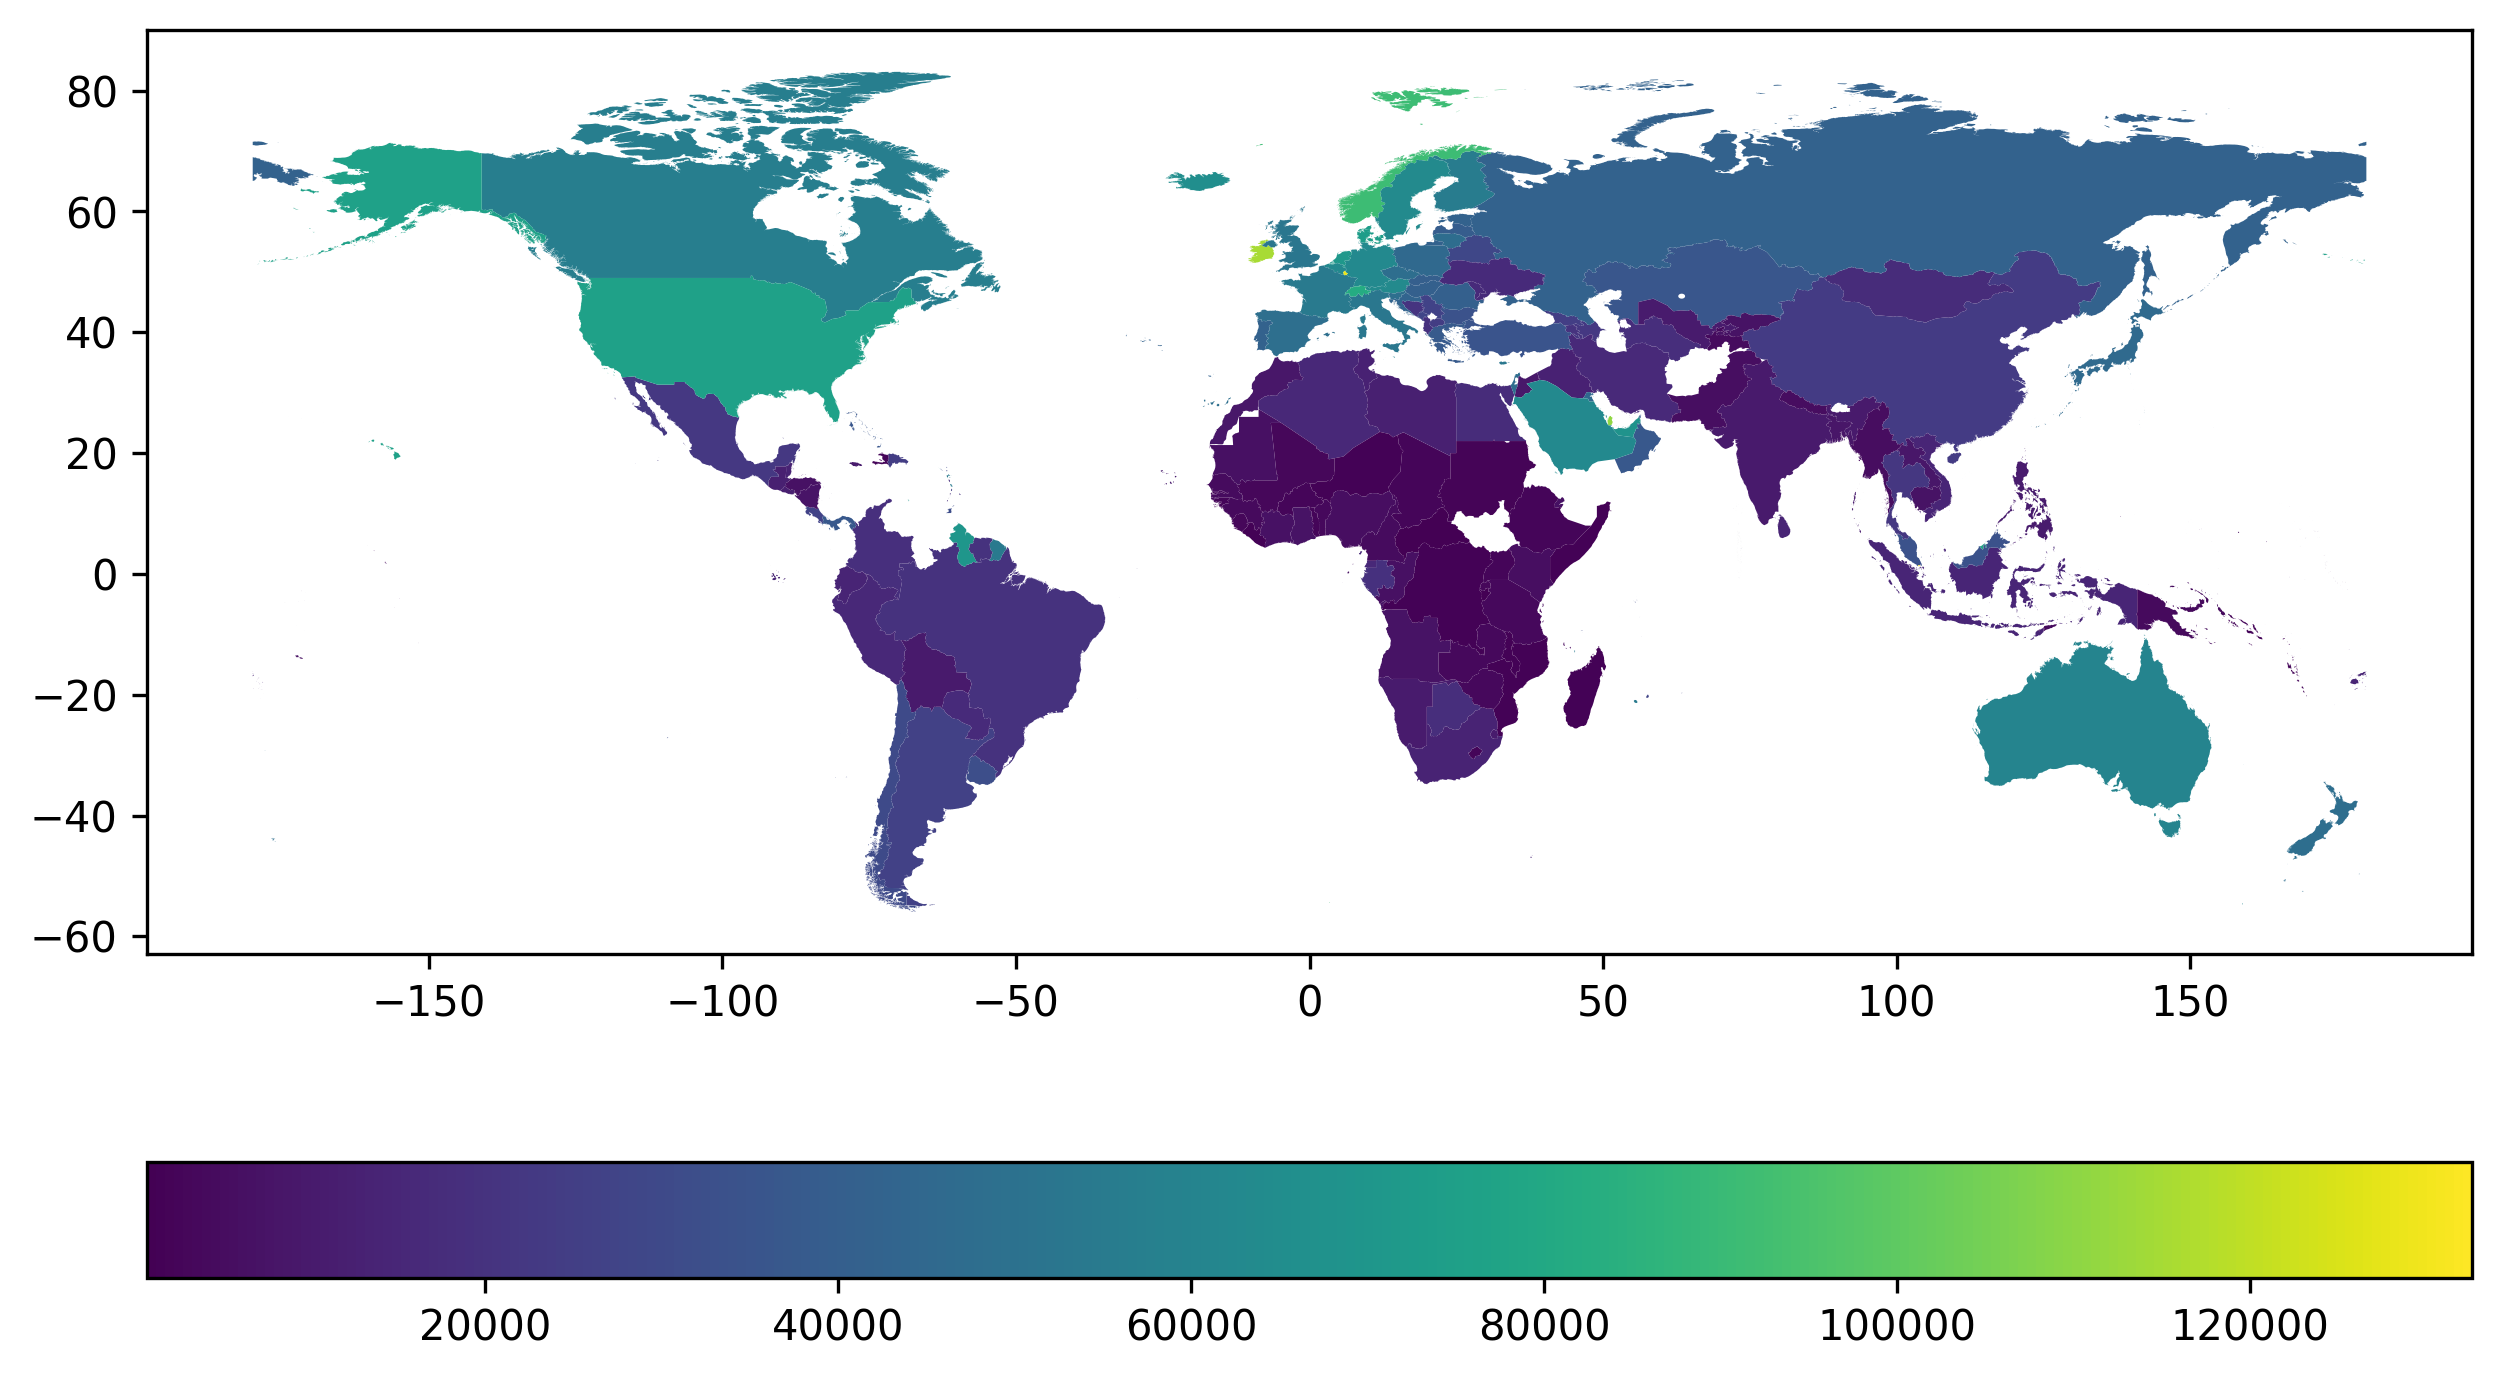
\includegraphics[width=1\linewidth]{figuras/pib/mapa_coropleto_paises_pib_percapita_ppc}
	\label{fig:mapa_coropleto_paises_pib_percapita_ppc}
	\footnotesize{Fonte: \cite{WB_pib_per_capita_países}.}
\end{figure}


Com base nos parágrafos anteriores e nas figuras, um questionamento surgiu: qual é relação entre EGDI e \textbf{E-Participation Index} com o PIB \textit{per capita} e com os gastos públicos (\% do PIB). Para descobrir qual tipo de coeficiente de correlação usar, fez-se diagramas de dispersão. Caso haja linearidade, usar-se-á Pearson; caso contrário, Spearman.

\subsubsection{Análise do EGDI, seus componentes e E-Participation Index}

Analisar-se-á o aspecto geral usando o EGDI, e seus componentes, e o \textbf{E-Participation Index}, estudando como essas variáveis se comportam em diagramas de dispersão e coeficientes de correlação quando comparada com outras variáveis.

\textbf{CONTINUAR AQUI}
